\documentclass[12pt,fleqn,answers]{exam}
\usepackage{pifont}
\usepackage{dingbat}
\usepackage{amsmath,amssymb}
\usepackage{epsfig}
\usepackage[colorlinks=true,linkcolor=black,anchorcolor=black,citecolor=black,filecolor=black,menucolor=black,runcolor=black,urlcolor=black]{hyperref}
\usepackage[letterpaper, margin=0.75in]{geometry}
\usepackage{tikz}
\usepackage[super]{nth}
\usetikzlibrary{arrows}
\addpoints
\boxedpoints
\pointsinmargin
\pointname{pts}

\usepackage{pdfpages}
\usepackage[final]{microtype}
\usepackage[american]{babel}
\usepackage[T1]{fontenc}
\usepackage{fourier}
%\usepackage{eucal}

\usepackage{isomath}
\usepackage{upgreek,amsmath}
\usepackage{amssymb}
\usepackage{siunitx}

\newcommand{\dotprod}{\, {\scriptzcriptztyle
    \stackrel{\bullet}{{}}}\,}

\newcommand{\reals}{\mathbf{R}}
\newcommand{\lub}{\mathrm{lub}} 
\newcommand{\glb}{\mathrm{glb}} 
\newcommand{\complex}{\mathbf{C}}
\newcommand{\dom}{\mbox{dom}}
\newcommand{\range}{\mbox{range}}
\newcommand{\cover}{{\mathcal C}}
\newcommand{\integers}{\mathbf{Z}}
\newcommand{\degree}{\mathrm{degree}}
\newcommand{\vi}{\, \mathbf{i}}
\newcommand{\vj}{\, \mathbf{j}}
\newcommand{\vk}{\, \mathbf{k}}
\newcommand{\bi}{\, \mathbf{i}}
\newcommand{\bj}{\, \mathbf{j}}
\newcommand{\bk}{\, \mathbf{k}}
\newcommand{\dist}{\, \mathrm{dist}}
\DeclareMathOperator{\Arg}{\mathrm{Arg}}
\DeclareMathOperator{\Ln}{\mathrm{Ln}}
\newcommand{\imag}{\, \mathrm{i}}

\usepackage{tikz}
\usepackage{amsmath}
\usetikzlibrary{arrows}
\usepackage{xcolor}
\shadedsolutions
\definecolor{SolutionColor}{rgb}{0.95,0.95,0.95}

\usepackage{graphicx}
\newcommand\AM{{\sc am}}
\newcommand\PM{{\sc pm}}
     
%\usepackage{twemojis}
\newcommand{\quiz}{15}
\newcommand{\term}{Spring}
\newcommand{\due}{9:55 \AM}
\newcommand{\class}{MATH 102}
\begin{document}
\large
\vspace{0.1in}
\noindent\makebox[3.0truein][l]{\textbf{\class, \term \/ \the\year}}
\textbf{Name:} \hrulefill \\
\noindent \makebox[3.0truein][l]{\textbf{In class work \quiz}}
\textbf{Row and Seat}:\hrulefill\\
%\vspace{0.1in}

%\small
\begin{flushleft}
  \emph{
 %   “Money buys everything except love, personality, freedom, immortality, silence, peace.”}
 %   \hfill \sc{Carl Sandburg}
  %  “Sometimes it's a little better to travel than to arrive.”}  \hfill {\sc  Robert M. Pirsig}
    “Self-education is, I firmly believe, the only kind of education there is.” 
    \hfill {\sc  Isaac Asimov }}
\end{flushleft}
 \large
%\noindent  In class work  \quiz\/  has questions 1 through  \numquestions \/ with a total of  \numpoints\/  points.   
% This assignment is due at the end of the class period (\due).
%This assignment is printed on \textbf{both} sides of the paper.
%\vspace{0.1in}


\begin{questions} 

\question Given that $F$ is a sequence and that $F_1 = 5, F_2 = 8$, and $F_3 = 42$.
Is $F$ an  \emph{arithmetic} sequence? Explain.

\begin{solution}[2.25in] No, $F$ is not an arithmetic sequence. To be an
  arithmetic sequence, the \emph{difference} of consecutive terms must be constant.
  But we have $F_2 - F_1 \neq F_3 - F_2$, so $F$ is not an arithmetic sequence.

\end{solution}

\question Given that $Q$ is a sequence and that $Q_1 =2, Q_2 = 8$, and $Q_3 = 42$.
Is $Q$ a  \emph{geometric} sequence? Explain.

\begin{solution}[2.25in] No, $Q$ is not a geometric sequence. To be a
  geometric  sequence, the \emph{quotient} of consecutive terms must be constant.
  But we have  $\frac{F_2}{F_1}\neq \frac{F_3}{F_2}$, so $Q$ is not a
  geometric sequence.


\end{solution}

\question Given that $G$ is an \emph{arithmetic} sequence and that $G_2 = 8$ and $G_4=9$, 
find a \emph{formula} for $G$.

\begin{solution}%^[2.25in]
  Since $G$  is an \emph{arithmetic} sequence its formula has the form $G_n = a n  + b$,
  where $a$ and $b$ are real numbers. Pasting in the given data, we have
  \begin{align*}
     8 &= 2 a + b, \\
     9 &= 4 a + b.
  \end{align*}
Solving for $a$ and $b$, we have $a=\frac{1}{2}$ and $b=7$. So a formula for $G$ is
$G_n = \frac{1}{2} n + 7$.

\end{solution}
%\vfill
%\newpage
    
\question Given that $H$ is a \emph{geometric} sequence and that $H_2 = 8$ and $H_4=9$, 
find a \emph{formula} for $H$.

\begin{solution}[2.25in]
  Since $H$ is a geometric sequence, its formula has the form $H_n = c a^n$, where $c$ 
  and $a$ are real numbers. Pasting in the given data, we have
  \begin{align*}
      8 &= c a^2 \\
      9 &= c a^4    
  \end{align*}
  Dividing the second equation by the first, we get 
  \begin{equation*}
     \frac{9}{8} = \frac{c a^4}{c a^2} = a^2.
  \end{equation*}
 So $a = \pm \sqrt{\frac{9}{8}}$. We were asked for a formula for $H$, not a representation
 of all possible formulae. So let's be positive and choose $a = \sqrt{\frac{9}{8}}$.
 
 Pasting  in $\sqrt{\frac{9}{8}}$ for $a$ in
 the first equation gives $8= \frac{9}{8} c $. So $c = \frac{64}{9}$ All together,
 \begin{equation*}
     H_n =  \frac{64}{9} \left(\sqrt{\frac{9}{8}}\right)^n.
 \end{equation*}
 Likely we should simplify this to something like
 \begin{equation*}
  H_n =  \frac{64}{9} \left(\frac{9}{8}\right)^{n/2}.
\end{equation*}
But there are forms that are acceptable.
\end{solution}

\question Find the \emph{numerical value} of each sum
\begin{parts}
  \part $\displaystyle \sum_{k=1}^{46} 1$
  \begin{solution}[1.25in]
  \begin{equation*}
    \sum_{k=1}^{46} 1 = 1 + 1 + \cdots + 1 = 46.
  \end{equation*}
  \end{solution} 

  \part $\displaystyle \sum_{k=1}^{107} (2 k + 3)$
  \begin{solution}[1.25in]
  \begin{align*}
    \sum_{k=1}^{107} (2 k + 3) &= \left(\sum_{k=1}^{107} 2 k \right)  + 
    \left(\sum_{k=1}^{107} 3 \right) &\mbox{(additivity)} \\
    &= \left(2 \sum_{k=1}^{107} k \right)  + 
    \left(3 \times 107\right) &\mbox{(outative)}\\
    &= 2 \times \frac{107 \times 108}{2} + 3 \times 107 &\mbox{(QRS)}\\
    &= 11877.
  \end{align*}
  \end{solution} 
\end{parts}

\question Given that $W$ is an \emph{arithmetic sequence} and that $W_1=2$ and $W_2 = 3$,
find the numerical value of $\displaystyle \sum_{k=1}^{42} W_k$. 

\begin{solution}%[2.25in]

  Since $W_k = a k + b$.  Pasting in the data, we have $2 = a + b$ and $3 = a + 2 b$. 
  Solving for $a$ and $b$ yields $a=1$ and $b=1$.  Now we need
  \begin{equation*}
    \sum_{k=1}^{42} W_k = \sum_{k=1}^{42} (1+k) = 42 + \frac{42 \times 43}{2} = 945.
  \end{equation*}

\end{solution}
%\vfill
%\newpage
\question After graduation from UNK, you expect a first year salary of $\$70,000$
and you expect a raise of 4\% for each of the 42 years that you plan to work. Your salary
for your $\mbox{n}^{\mbox{th}}$ year of work $S_n$ is
\begin{equation*}
    S_n = 70000 \times 1.04^{n-1}
\end{equation*}

\begin{parts}
  \part Find the numerical value of $S_{42}$. This is your salary the year you retire.
  \begin{solution}[1.25in]
     \begin{equation*}
        S_{42} = 70000 \times 1.04^{41} = 349,514.30.
     \end{equation*}

  \end{solution} 

  \part Over your career, your total earnings will be
  \begin{equation*}
       \sum_{k=1}^{42} 70000 \times 1.04^{k-1}.
  \end{equation*}
  Find the numerical value of your total earnings.
\end{parts}
\begin{solution}[1.25in]
  This one is a bit tricky. To match the sum to the geometric sum in the QRS,
  we need to use the trick $1.04^{k-1} = \frac{1.04^k}{1.04}$. We have
  \begin{align*}
    \sum_{k=1}^{42} 70000 \times 1.04^{k-1}&=
    \sum_{k=1}^{42} 70000 \times \frac{1.04^k}{1.04}\\
    &= \frac{70000}{1.04} \sum_{k} 1.04^k\\
    &=\frac{70000}{1.04} \frac{1.04^{43} - 1.04}{1.04-1}
    =7,337,371.84.
  \end{align*}
You all can expect to earn about seven million dollars in your lifetime.
\end{solution} 

\hfil
\newpage
\question The human population $P$ of Floyd, Virginia is an exponential function of the years $T$ after the year 2000.  Specifically,
the population in the years 2000 and 2010 are given in the table

\begin{figure*}[h]
\begin{center}
\begin{tabular}{|c|c|c|} \hline
  Year & $T$  & $P$ \\ \hline
  2000 & 0    & 432  \\
  2010 & 10   & 425  \\ \hline
  \end{tabular}.
  \caption{Human population of Floyd for the years 2000 and 2010.}
  \end{center}
\end{figure*}
\begin{parts}

\part [2] Find the exponential function that matches the given data.

\begin{solution}[2.0in] We just need to match to the general result in the QRS. That gives
   \begin{equation*}
       P = 432 \times \left(\frac{425}{432} \right)^{T/10}.
   \end{equation*}
\end{solution}

\part [2] Using your exponential function from part `a,' when will the population of Floyd be 250?

\begin{solution}[3.0in] 
   We need to solve $250 = 432 \times \left(\frac{425}{432} \right)^{T/10}$ for $T$. Some (many) students will be more comfortable
   using decimal approximations to various quotients as they go. That's OK.
   \begin{align*}
   \left[250 = 432 \times \left(\frac{425}{432} \right)^{T/10} \right] &=
   \left[\frac{250}{432} = \left(\frac{425}{432} \right)^{T/10} \right] &\mbox{($\div$ 432)} \\
   &= \left[\log(\frac{250}{432}) = \log \left(\left(\frac{425}{432} \right)^{T/10} \right) \right] &\mbox{(log of left and right)} \\
   &= \left[\log \left (\frac{250}{432} \right) = \frac{T}{10} \log \left(\frac{425}{432}  \right) \right] &\mbox{(log property)} \\
   &= \left[T = 10 \times \frac{\log \left (\frac{250}{432} \right)}{\log \left(\frac{425}{432} \right)} \right], &\mbox{(divide)} \\
   &= \left[T \approx 334  \mbox{ years} \right]. 
   \end{align*}
This is so far into the future, it's almost surely wildly inaccurate.
\end{solution}

\end{parts}

%\hfill
%\newpage


\question [2]  Find the solution to the linear equations
\begin{align*}
   5 x + 8 y &= 14, \\
   x -  y &= 3.
\end{align*}

\begin{solution}[3.0in] Let's use our matrix method. Ordering the unknowns as $x$  (first column) and $y$ (second column), 
   our system in matrix form is
   \begin{align*}
       \begin{bmatrix} 5 & 8 & 14 \\ 1 & -1 & 3 \end{bmatrix}
       \begin{bmatrix}  \\  & R_2 \leftarrow R_1 - 5 R_2 \end{bmatrix}
       &= \begin{bmatrix} 5 & 8 & 14 \\ 0 & 13 & -1 \end{bmatrix}
   \end{align*}
   The second equation is $13 y = -1$. So $y=-\frac{1}{13}$. Pasting that into the 
   first equation gives $5 x - \frac{8}{13} = 14$. So $x = \frac{38}{13}$. 

   Should we check our work?  Sure. 
   \begin{equation*}    
      \left[5 x + 8y = 14\right] = \left[5 \times \frac{38}{13} - 8 \times \frac{1}{13} = 14\right] =
     \mbox{True!}      
   \end{equation*}
   And one more time
   \begin{equation*}    
      \left[x - y = 3\right] = \left[\frac{38}{13}  + \frac{1}{13} = 3 \right] 
      = \mbox{True!}      
   \end{equation*}
\end{solution}

\question [2] Find the solution to the linear equations
\begin{align*}
   x + y + z &= 6, \\
   y + z &= 10,\\
   y - z &= 20.
\end{align*}

\begin{solution}[2.5in]
  $  x=-4,y=15,z=-5$
\end{solution}

\question [2] Larry is saving his money to purchase a
1968 Fender Stratocaster Sunburst guitar.
To save for the guitar, he invests \$5,000 into a bank CD with an APY of 5.0\%. 
How long will Larry need to wait until he can purchase the 1968 Stratocaster that costs
\$7,700?

\begin{solution}%[3.0in]
    We need to solve $7700 = 5000 \times 1.05^T$ for $T$. Since the unknown
    $T$ is an exponent, we'll use the \emph{logarithm trick}. Specifically,
    \begin{align*}
      \left[7700 = 5000 \times 1.05^T \right] &= \left[1.54 = 1.05^T \right], &\mbox{(divide by 5000)} \\
                     &= \left[\log_{10}(1.54) = \log_{10}(1.05^T) \right],  &\mbox{(logarithm trick)} \\
                     &= \left[\log_{10}(1.54) = T \log_{10}(1.05) \right],  &\mbox{(logarithm property)} \\
                     &= \left[ T = \frac{\log_{10}(1.54)}{\log_{10}(1.05)} \right],  &\mbox{(divide by $\log_{10}(1.05)$)} \\
                     &= \left[ T \approx 8.85 \mbox{ years} \right].  &\mbox{(arithmetic)}
    \end{align*}

\end{solution}

%\vfill
%\newpage
\question [2] In April 2003, Ms Oro purchases one ounce of gold for \$647. 
Today (that is, twenty years later), Ms Oro sells her gold for \$1,995.
Find the APY for this investment.
\begin{solution}[3.0in]
We need to solve $1995 = 647 \times (1+r)^{20}$ for $r$. Since 
the unknown is in the base of an exponential, we use the \emph{root trick}.
Specifically,
\begin{align*}
    \left[1995 = 647 \times (1+r)^{20} \right] &= \left[\frac{1995}{647} = (1+r)^{20} \right], & \mbox{(divide by 647)}\\
               &= \left[\left(\frac{1995}{647}\right)^{1/20} = (1+r) \right], & \mbox{(root trick)} \\
               &= \left[r = \left(\frac{1995}{647}\right)^{1/20} - 1 \right], & \mbox{(subtract 1)}\\
               &= \left[ r \approx 5.79\% \right]. &\mbox{(arithmetic)}
\end{align*}
You might be more comfortable doing the arithmetic as you go, instead
of saving it up until the end. That's okay, but I think it makes it
more difficult to check the work, increases chances of miscopying
numbers, and it potentially decreases accuracy (by rounding intermediate results).
Try saving the arithmetic to the end--you might like it.

\textbf{FYI:} By investing in a stock index fund, Ms Oro would have
gotten a higher APY on her investment. For the cost of gold, I used 
actual historical data--I didn't just make it up.

And by the way: the Spanish word for gold is `oro.'


\end{solution}


\question To save for the purchase of a new 781 Porsche Boxster,
Morweena purchases a bond with a value of \$80,000 when it matures
in 20 years.

\begin{parts}

    \part [2] At the time of purchase, the 20 year APY is 5.0\%.
    Find the \emph{purchase price} of the bond.
    \begin{solution}[3.0in] We need to solve 
        $80000 = P \times 1.05^{20}$ for $P$. We have
        \begin{equation*}
             P = \frac{80000}{1.05^{20}} \approx 30151.16.
        \end{equation*}

    \end{solution}

    \part [2] After five years, Morweena decides to sell her bond and
    to use the proceeds to purchase an organic vanilla bean farm in Hawaii.
    At the time of sale, the 20 year APY is 4.0\%. Find the 
    sale price of the bond.
    \begin{solution}[3.0in] The future value of the bond is still
        \$80,000. Think of it this way: if you purchase the bond from 
        Morweena and hold onto it until maturity, the Federal government
        will pay you \$80,000. So its future value is still \$80,000.        
        What has changed is both the time to maturity (was
        20 years, now is 15) and the APY is 4.0\% .
        We now need to solve $80000 = P \times 1.04^{15}$ for $P$. 
        We have
        \begin{equation*}
             P = \frac{80000}{1.04^{15}} \approx 44421.160.
        \end{equation*}

  


    \end{solution}




\end{parts}

\question A sequence $J$ is defined by 
\begin{equation*}
   J_n = \begin{cases} 1 & n=1 \\ J_{n-1} + 1 & n \geq 2 \end{cases}.
\end{equation*}
Find the \emph{numerical value} of $J_4$.

\begin{solution}
  \begin{align*}
    J_1 &= 1 &\mbox{(given explicitly by formula)} \\
    J_2 &= J_1 + 1 = 1 + 1 = 2, \\
    J_3 &= J_2 + 1 = 2 + 1 = 3, \\
    J_4 &= J_3 + 1 = 3 + 1 = 4.
  \end{align*}

\end{solution}

\end{questions}
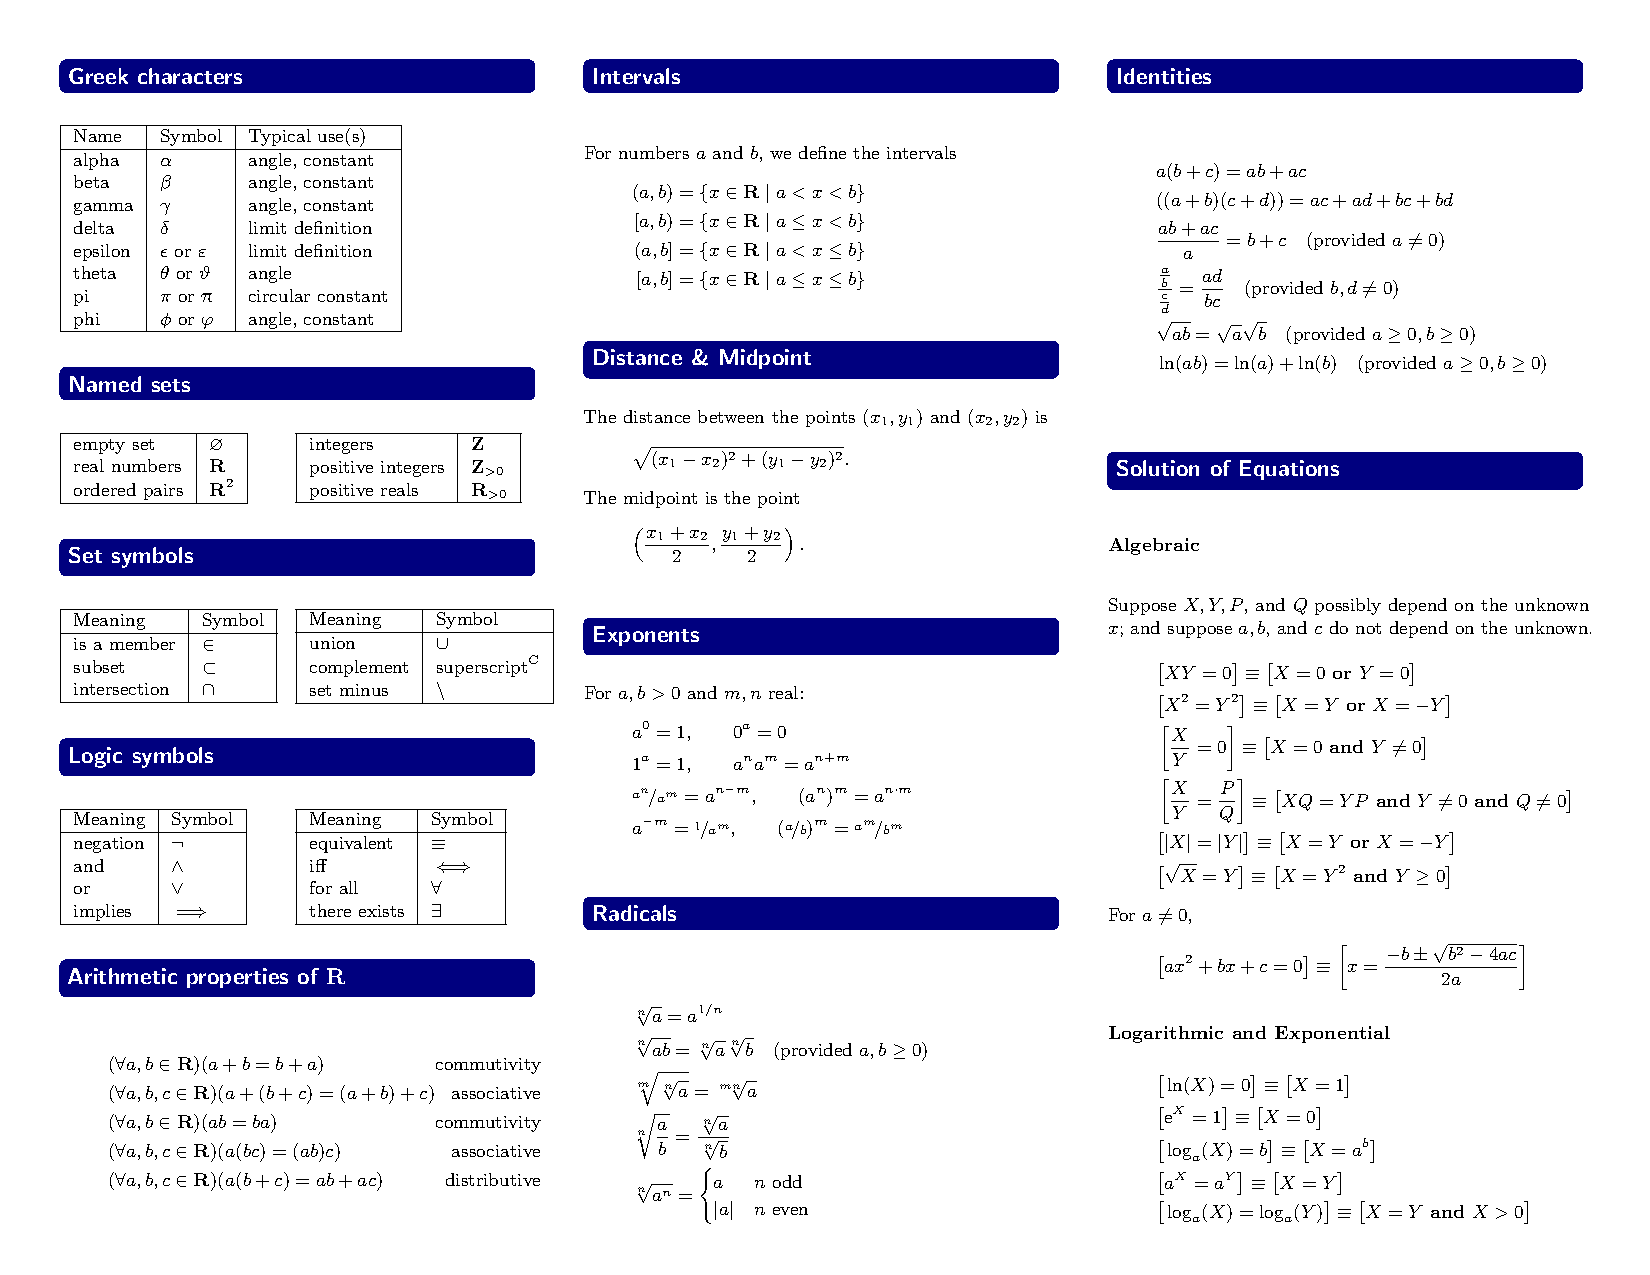
\includepdf[pages=-]{college-algebra-quick-reference}
\end{document}
